\begin{frame}[plain]
\frametitle{The Data Plane is continuously evolving.}
\begin{itemize}
\item Progression of queue-management/scheduling algorithms:
\begin{itemize}
\item WFQ, SFQ, RED, BLUE, ECN, XCP, RCP, CoDel, pFabric
\end{itemize}
\item Each scheme wins in its own evaluation.
\item Tacit belief in knobless queue management/scheduling
\end{itemize}
\end{frame}

\begin{frame}[plain]
\frametitle{Yet, there is no silver bullet.}
\begin{itemize}
\item{Different applications care about different things.}
%%\begin{itemize}
%%\item Interactive video conferencing apps need both high throughput \& low delay.
%%\item Bulk transfers care only about high throughput.
%%\item Web browsers care about minimizing flow completion time (FCT).
%%\end{itemize}

\item{Applications use different transport protocols.}
%%%\begin{itemize}
%%%\item Some respond to loss, e.g., TCP Cubic, TCP NewReno.
%%%\item Others respond to packet inter-arrival times, e.g., WebRTC, LEDBAT.
%%%\item Others respond to per-packet delay, e.g., TCP Vegas.
%%%\item Yet others respond to both delay and packet loss, e.g., Compound TCP.
%%%\end{itemize}

\item{Diversity in network conditions.}
%%\begin{itemize}
%%\item High-speed, low-latency, Data Center networks
%%\item Low-speed, high-latency, transcontinental links
%%\item High-speed, high-variability, bufferbloated LTE links
%%\end{itemize}
\item{``One size fits all'' is overly constraining.}
\end{itemize}
\end{frame}

\begin{frame}[plain]
\frametitle{Quantifying ``No Silver Bullet'': Network configurations}
Network Configurations:
\begin{table}
\begin{tabular}{|p{0.25\linewidth}|p{0.73\linewidth}|}
\hline
{\bf Network Configuration} & {\bf Description} \\
\hline
{\bf CoDel+FCFS} & CoDel running on a single shared first-come, first-served queue.\\
\hline
{\bf CoDel+FQ} & A separate queue for each flow with an independent instance of CoDel running on each queue. Queues are serviced using fair queueing. \\
\hline
{\bf Bufferbloat+FQ} & A separate queue for each flow with a deep buffer that doesn't drop any packets. Queues are serviced using fair queueing. \\
\hline
\end{tabular}
\end{table}
\end{frame}

\begin{frame}[plain]
\frametitle{Quantifying``No Silver Bullet'': Simulation Workloads}
%\frametitle{Quantitative evidence for ``No Silver Bullet''}
Workloads:
\begin{table}
\begin{tabular}{|p{0.15\linewidth}|p{0.39\linewidth}|p{0.38\linewidth}|}
\hline
{\bf Workload} & {\bf Description} & {\bf Objective} \\
\hline
\textbf{\emph{Bulk}} & Long-running TCP flow. & Maximize average throughput. \\
\hline
\textbf{\emph{Web}} & Switched TCP flow that alternates between ON and OFF periods. & Minimize flow completion time at the 99.9th percentile. \\
\hline
\textbf{\emph{Interactive}} & Long-running TCP flow representing a real-time interactive application. & Maximize the ratio of throughput and one-way delay, i.e., ``power.'' \\
\hline
\end{tabular}
\end{table}
\end{frame}

\begin{frame}[plain]
\frametitle{Quantifying ``No Silver Bullet'': Cyclic Preference Loops}
\textbf{No single network configuration is the best.} \\
\begin{center}
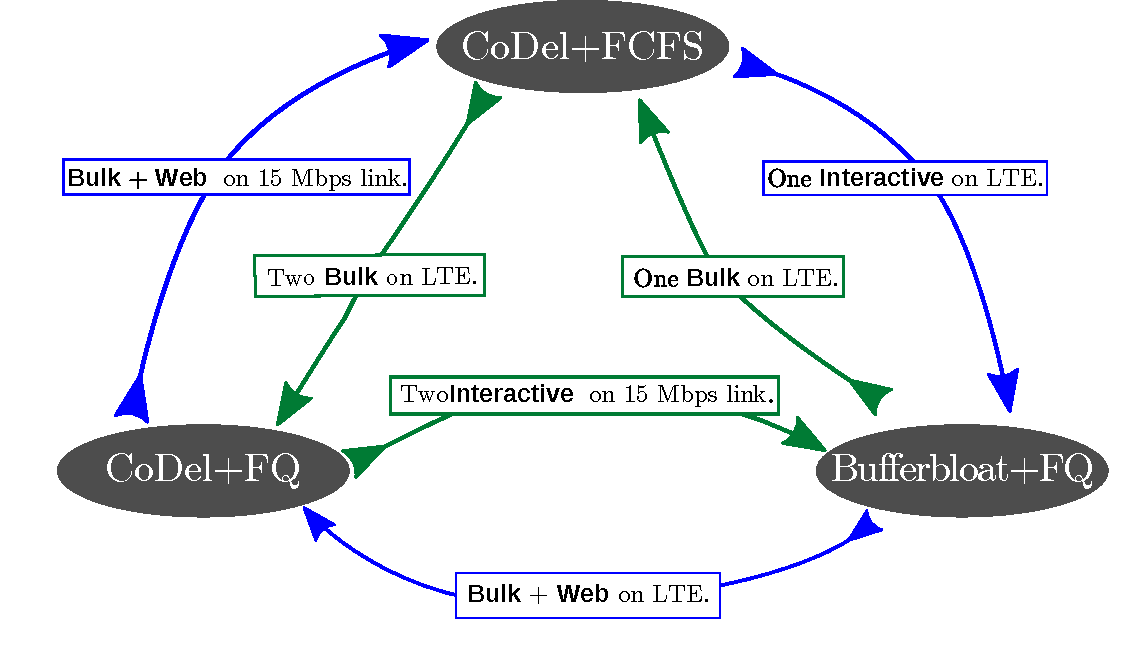
\includegraphics[width=\columnwidth]{fig.pdf}
\end{center}
\end{frame}

\begin{frame}[plain]
\frametitle{Explaining cyclic preferences}
\begin{itemize}
\item Dropping packets significantly degrades throughput.
      \begin{itemize}
      \item Reason: Variable-rate links have an inherent delay-throughput tradeoff, unlike static links.
      \end{itemize} 
 
\item FCFS is preferable to Fair Queuing in some cases.
      \begin{itemize}
      \item Reason: When equally aggressive flows compete, they don't need protection from each other.
      \end{itemize}

\item Fair Queuing is required in some cases.
      \begin{itemize}      
      \item Reason: When competing flows are not equally aggressive, they need isolation from each other.
      \end{itemize}
\end{itemize}
\end{frame}

\begin{frame}[plain]
\frametitle{The Solution}
Flexible Switch Data Planes
\begin{itemize}
\item No ``Silver Bullet'' queue-management/scheduling scheme
\item Application demands continue to evolve.
\item Networks supporting these applications will evolve as well.
\item The Data Plane should support newly developed schemes.
\end{itemize}
\end{frame}

\begin{frame}[plain]
\frametitle{But, do so in a controlled manner.}
\begin{itemize}
\item Provide interfaces to the head and tail of switch queues.
\item Operators specify only queue-management/scheduling logic.
\item Code size limits constrain program sophistication.
\item Disallow access to packet payloads.
\end{itemize}
\end{frame}

\begin{frame}[plain]
\frametitle{Re-architecting network switches for data plane programmability.}
\begin{itemize}
\item Hardware Primitives
      \begin{itemize}
      \item Random number generators
      \item Binary tree of comparators
      \item EWMA estimators
      \end{itemize}

\item I/O interfaces
      \begin{itemize}
      \item Access to head/tail of queue
      \item Drop from head/tail of queue
      \item Interrupts for enqueue/dequeue
      \item Reading packet fields
      \end{itemize}

\item State variables
      \begin{itemize}
      \item Per-flow
      \item For fastest flows alone
      \item Per-src address
      \end{itemize}

\item Instruction Set
      \begin{itemize}
      \item Express Control Flow
      \item Implement new functionality unavailable in hardware
      \end{itemize}
\end{itemize}
\end{frame}

\begin{frame}[plain]
\frametitle{Example implementation: CoDel}
\begin{center}
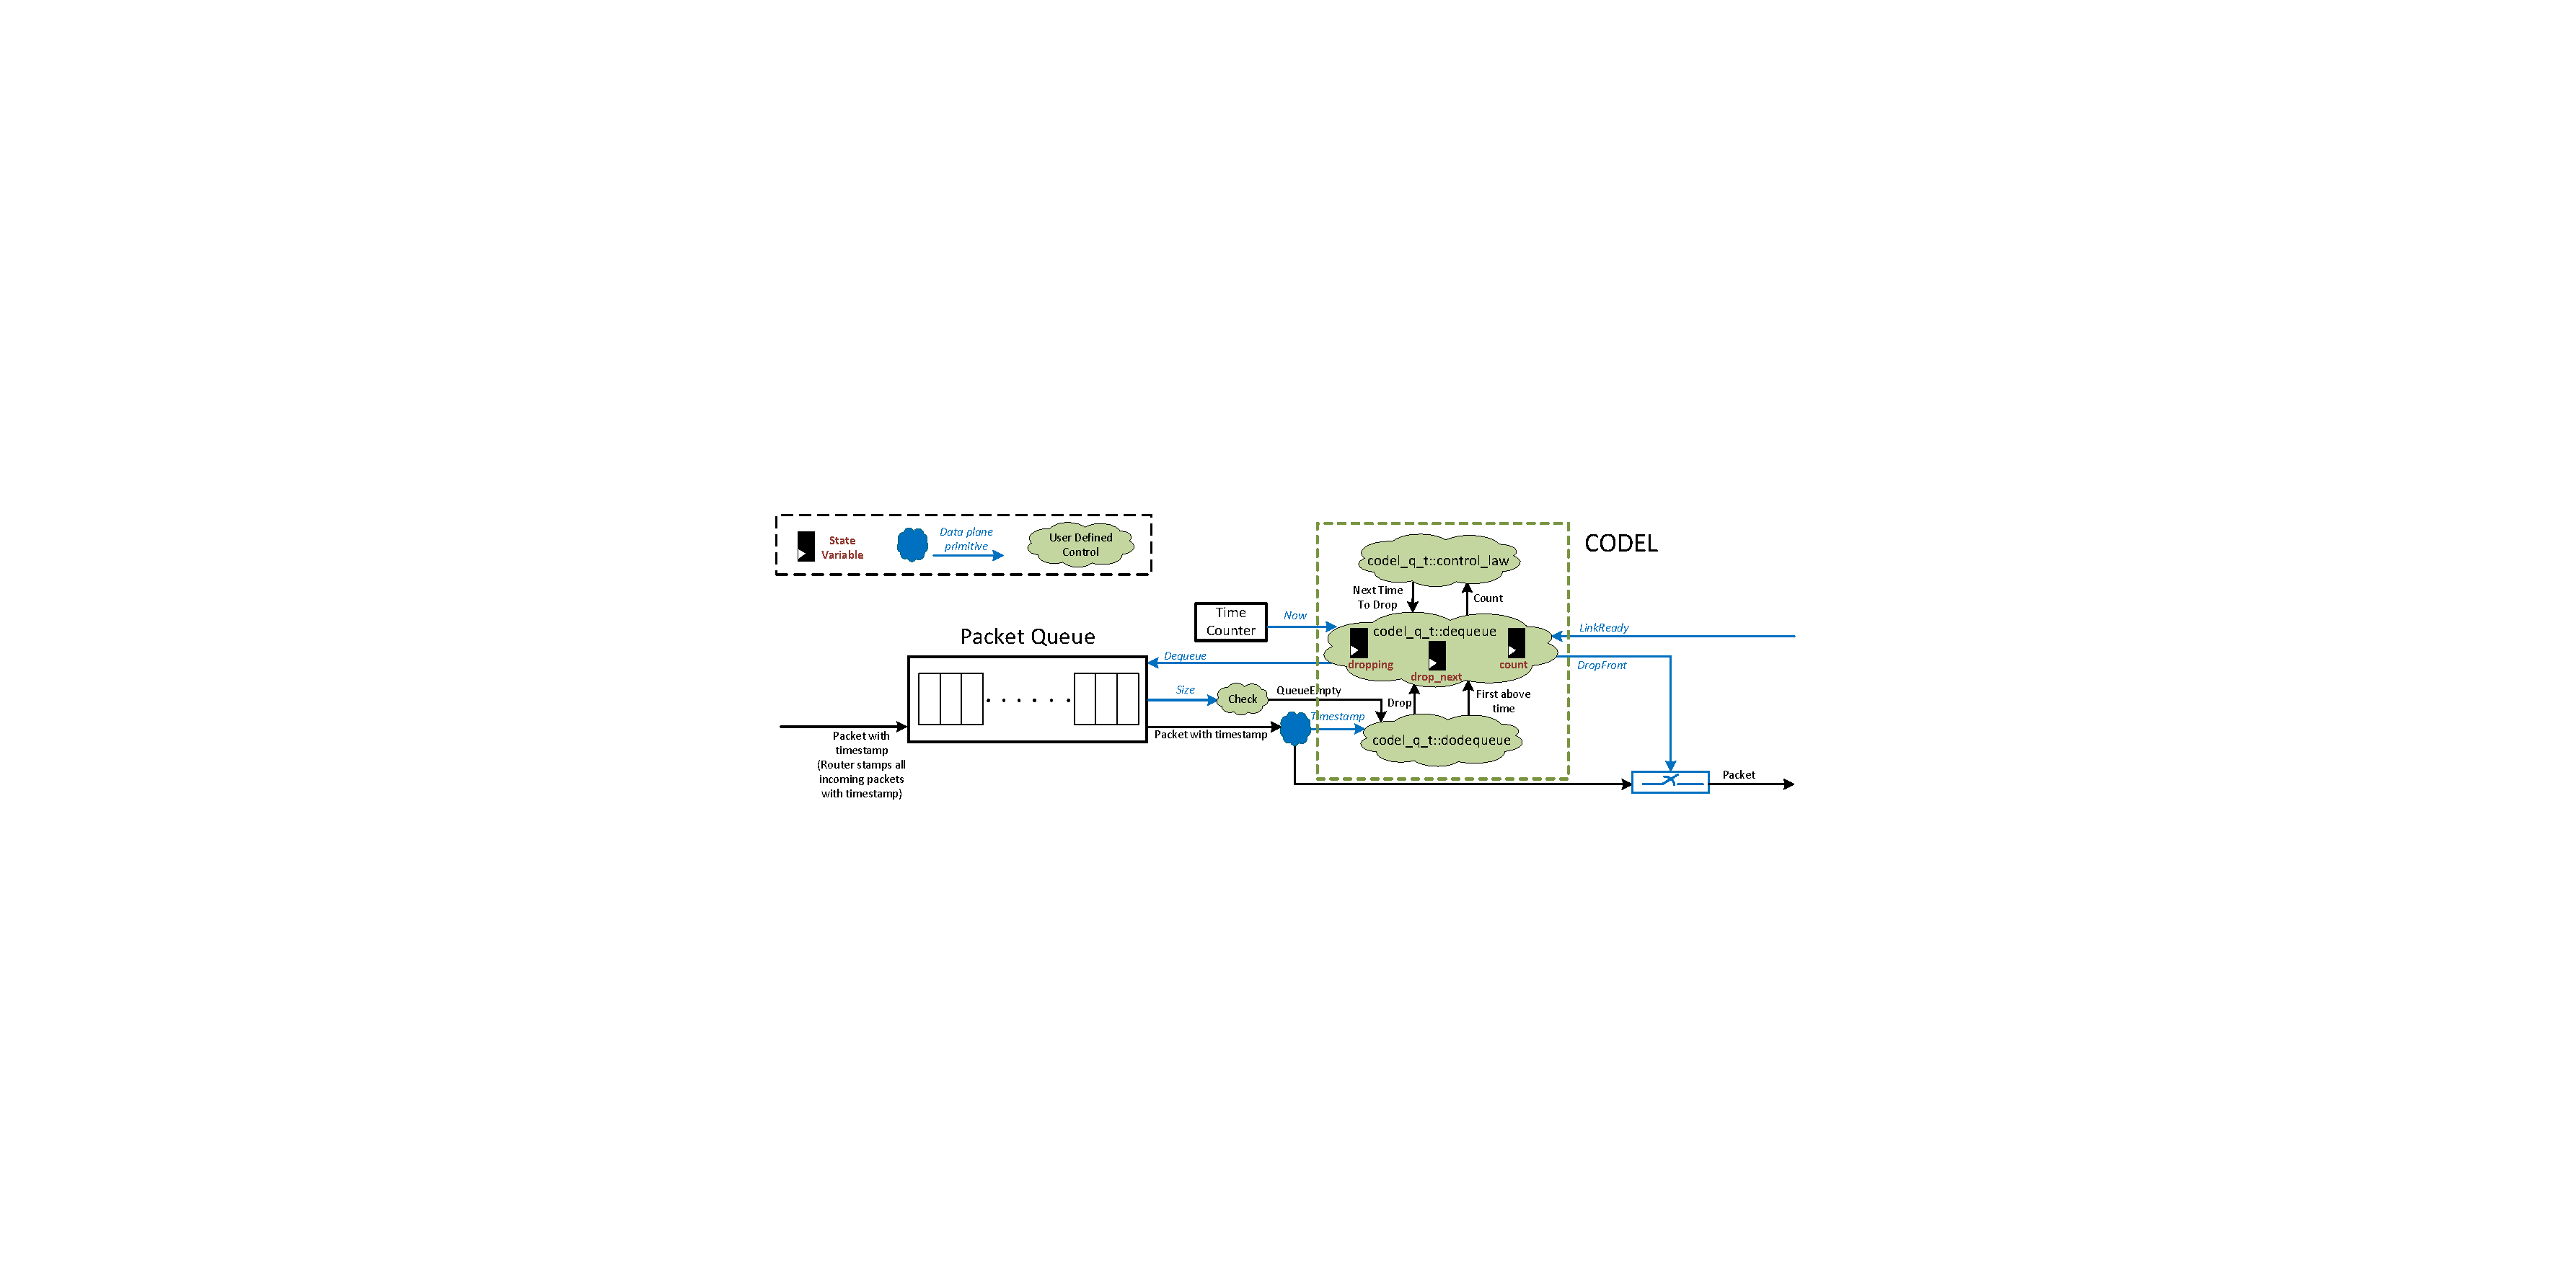
\includegraphics[width=\columnwidth]{codel.pdf}
\end{center}
\begin{center}
Synthesis numbers: \\
\begin{tabular}{lll}
\bf Resource & \bf Usage & \bf Fraction of FPGA \\
\hline Slice logic & 1,256 & 1\% \\
Slice logic dist. & 1,975 & 2\% \\
IO/GTX ports & 27 & 2\% \\
DSP slices & 0 & 0\% \\
Maximum speed & 12.9 $\times 10^6$ pkts/s \\
\end{tabular}
}
\end{center}
\end{frame}

%%%%%%%%\section*{A blueprint for a flexible Data Plane}
%%%%%%%%
%%%%%%%%\begin{itemize}
%%%%%%%%\item Standardized interfaces to the rest of the switch
%%%%%%%%
%%%%%%%%\begin{center}
%%%%%%%%
%%%%%%%%\begin{tabular}{|l|l|l|}
%%%%%%%%\hline
%%%%%%%%\bf Class of primitive & \bf Primitive Name & \bf Description \\
%%%%%%%%\hline
%%%%%%%%Utilities & $Now$ & Get current time. \\
%%%%%%%%\hline
%%%%%%%%Queue primitives & $Size$ & Get queue length. \\
%%%%%%%%\hline
%%%%%%%%Queue primitives & $DropFront$ & Drop packet from head of queue.  \\
%%%%%%%%\hline
%%%%%%%%Queue primitives & $DropTail$ & Drop packet from tail of queue. \\
%%%%%%%%\hline
%%%%%%%%Queue primitives & $Enqueue$ & Enqueue packet at tail of queue. \\
%%%%%%%%\hline
%%%%%%%%Queue primitives & $Dequeue$ & Dequeue packet from head of queue. \\
%%%%%%%%\hline
%%%%%%%%Queue primitives & $Transmit$ & Transmit single packet. \\
%%%%%%%%\hline
%%%%%%%%Signaling primitives & $LinkReady$ & Link is ready to accept packet. \\
%%%%%%%%\hline
%%%%%%%%Signaling primitives & $Arrival$ & New packet just arrived. \\
%%%%%%%%\hline
%%%%%%%%Packet primitives & $Timestamp$ & Packet's arrival timestamp. \\
%%%%%%%%\hline
%%%%%%%%Packet primitives & $Mark$ & Set ECN bit. \\
%%%%%%%%\hline
%%%%%%%%Cross-layer primitives & $LinkRates$ & Get current link rate. \\
%%%%%%%%\hline
%%%%%%%%\end{tabular}
%%%%%%%%\end{center}
%%%%%%%%
%%%%%%%%\item Add a small amount of reconfigurable logic to the switch.
%%%%%%%%\item Enforce hard resource limits on the amount of reconfigurable logic.
%%%%%%%%\item Express queuing/scheduling logic as code in a high-level language.
%%%%%%%%\end{itemize}
%%%%%%%%
%%%%%%%%\section*{Example implementation: CoDel}
%%%%%%%%
%%%%%%%%\begin{itemize}
%%%%%%%%\item Implemented CoDel in SystemVerilog.
%%%%%%%%\item Synthesized into gate-level netlist using Xilinx's freely available Vivado WebPacket compiler.
%%%%%%%%\item Block diagram of implementation:
%%%%%%%%\\
%%%%%%%%\begin{center}
%%%%%%%%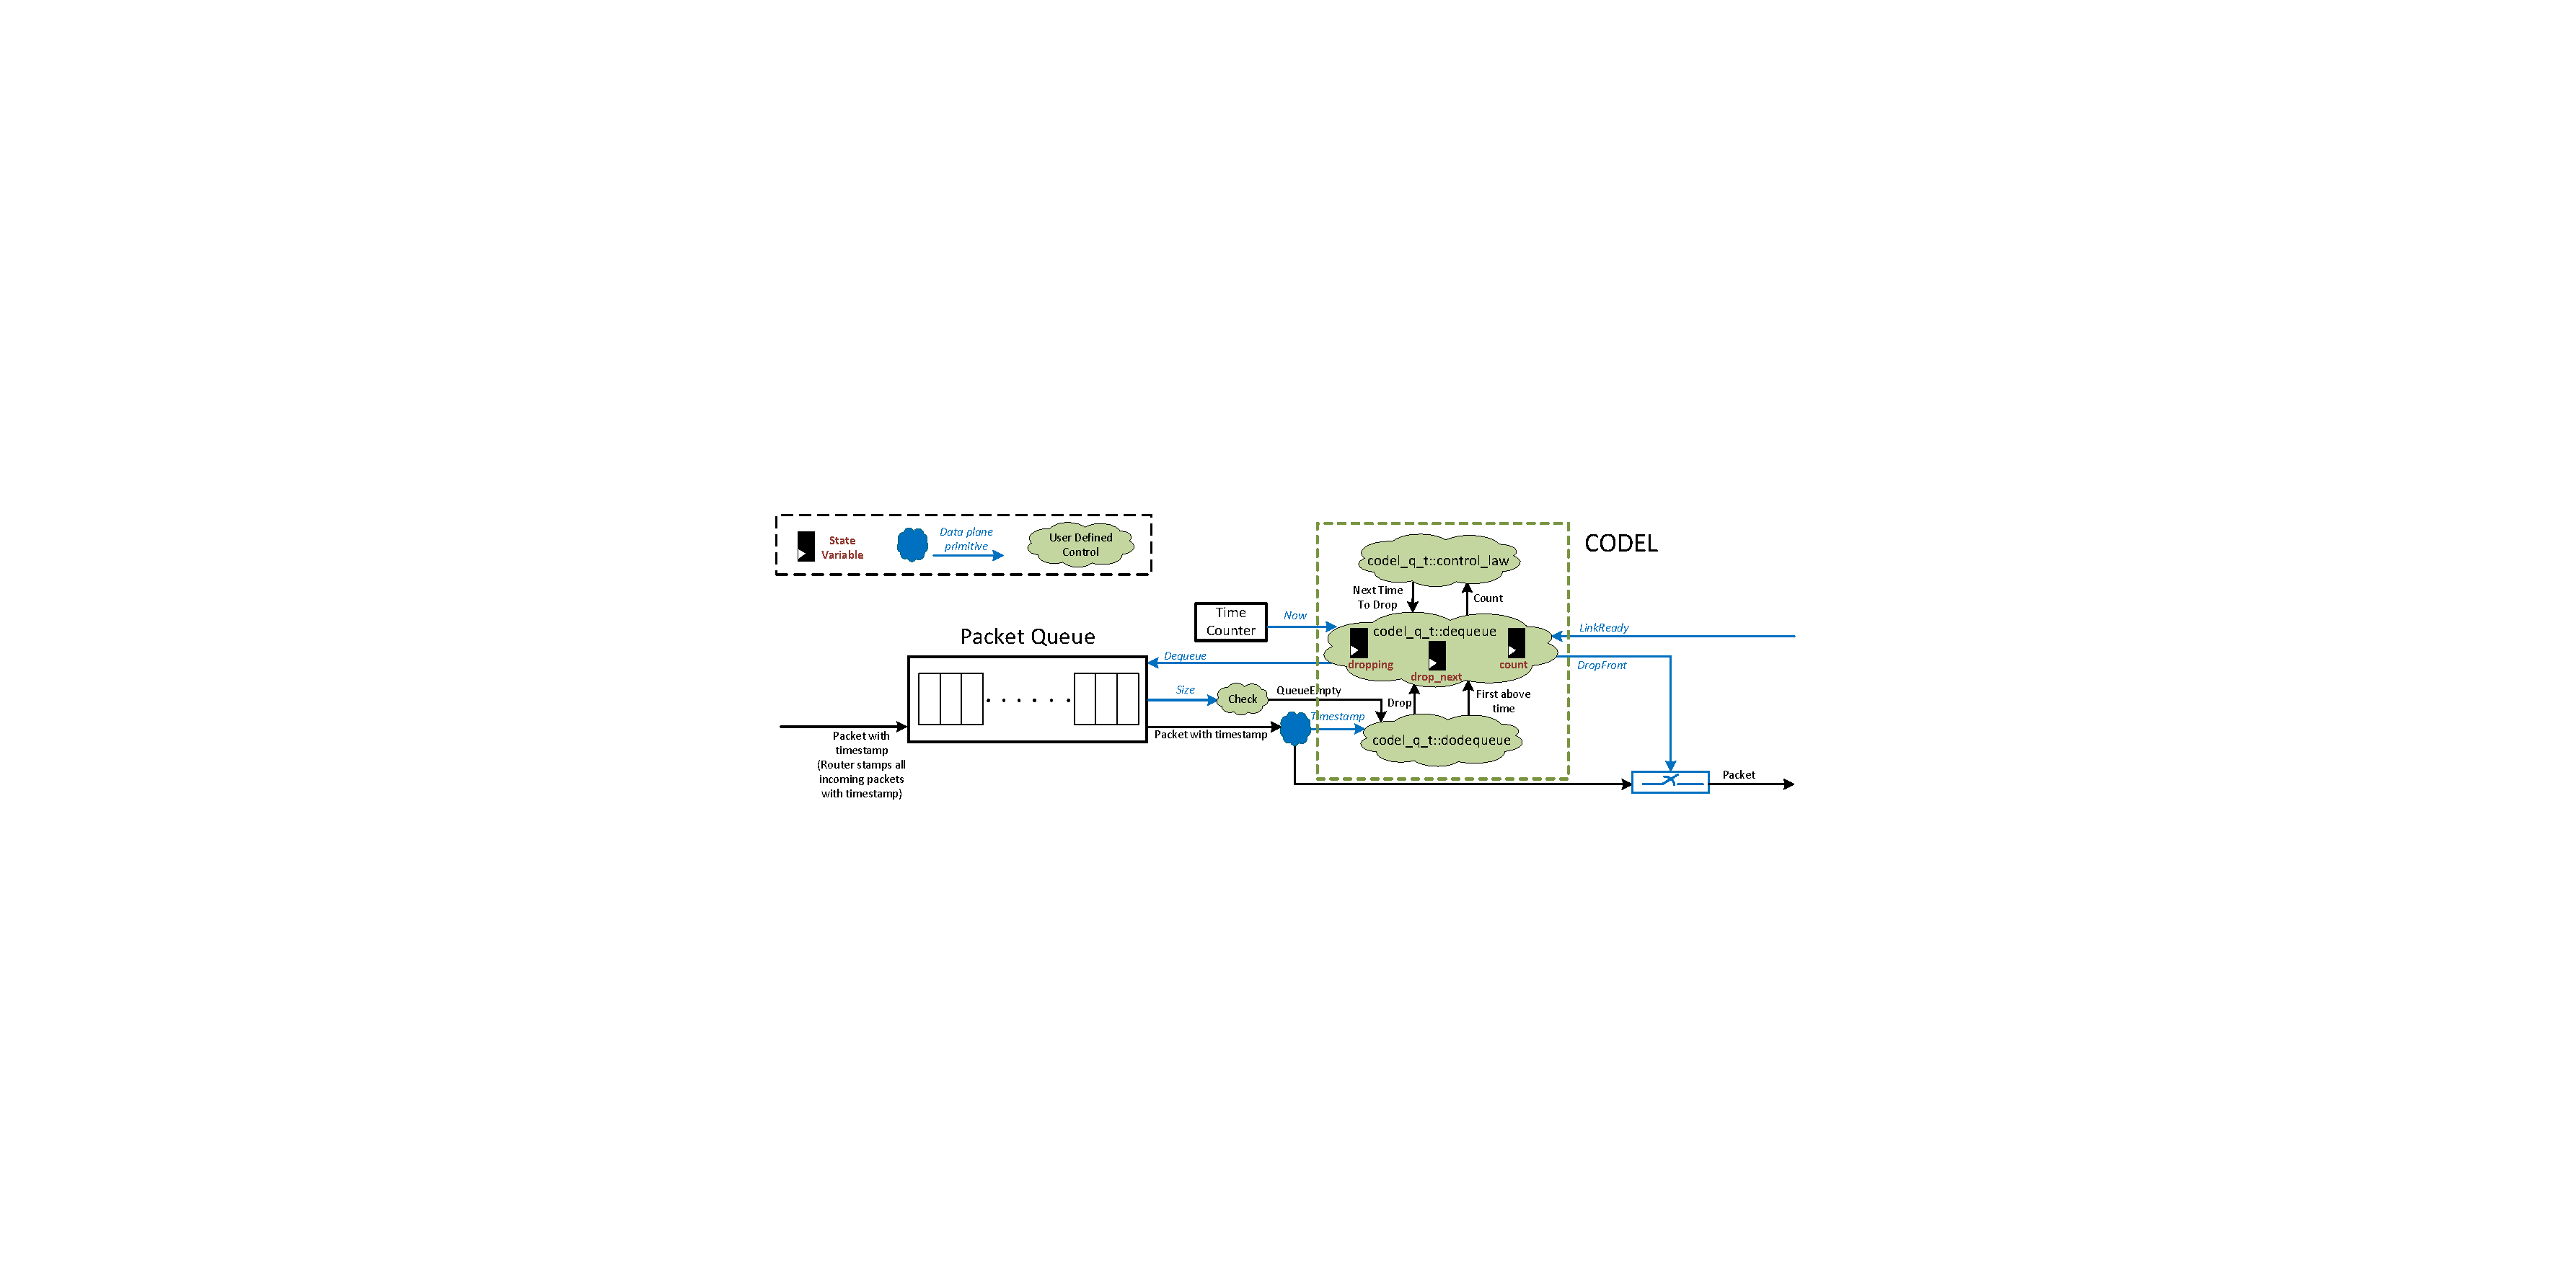
\includegraphics[width=\columnwidth]{codel.pdf}
%%%%%%%%\end{center}
%%%%%%%%\item \textbf{CoDel resource utilization on Xilinx Kintex-7:}\\
%%%%%%%%\begin{center}
%%%%%%%%\begin{tabular}{|l|l|l|}
%%%%%%%%\hline
%%%%%%%%\bf Resource & \bf Usage & \bf Fraction of FPGA \\
%%%%%%%%\hline Slice logic & 1,257 & 2\% \\
%%%%%%%%\hline Slice logic dist. & 1,969 & 4\% \\
%%%%%%%%\hline IO/GTX ports & 27 & 6\% \\
%%%%%%%%\hline DSP slices & 0 & 0\% \\
%%%%%%%%%\hline Maximum speed & 12.9 million pkts/s & N/A \\
%%%%%%%%\hline
%%%%%%%%\end{tabular}
%%%%%%%%\end{center}
%%%%%%%%\item Synthesized implementation passes timing checks at 12.9 million pkts/s
%%%%%%%%
%%%%%%%%\end{itemize}
%%%%%%%%
%%%%%%%%\section*{Limitations and Practical Considerations:}
%%%%%%%%\begin{itemize}
%%%%%%%%\item Cannot express several important network functions:
%%%%%%%%      \begin{itemize}
%%%%%%%%      \item ``Deep-packet'' Inspection
%%%%%%%%      \item Intrusion Detection
%%%%%%%%      \item Spam Filtering
%%%%%%%%      \end{itemize}
%%%%%%%%\item Mechanism for signaling application objectives to the network.
%%%%%%%%      \begin{itemize}
%%%%%%%%      \item Could use DiffServ codepoints.
%%%%%%%%      \item But ASes generally don't honor codepoints from other ASes.
%%%%%%%%      \item May be a non-issue inside a Data Center.
%%%%%%%%      \end{itemize}
%%%%%%%%\item Most switches today have a shared pipeline with demanding requirements.
%%%%%%%%      \begin{itemize}
%%%%%%%%      \item Top-of-the-line switches have 64 ports, each running at 10G.
%%%%%%%%      \item Implies that queueing/scheduling logic should run at 64*10G.
%%%%%%%%      \item If queue management is enqueue-based, e.g., RED, this problem cannot be fixed by replicating digital logic on each port.
%%%%%%%%      \end{itemize}
%%%%%%%%\item Mechanism to map flows onto per-port queues is required for scheduling.
%%%%%%%%      \begin{itemize}
%%%%%%%%      \item Also need to decide on the number of such queues.
%%%%%%%%      \end{itemize}
%%%%%%%%\item Interoperability
%%%%%%%%      \begin{itemize}
%%%%%%%%      \item Across switch vendors.
%%%%%%%%      \item Across FPGA vendors.
%%%%%%%%      \end{itemize}
%%%%%%%%\item Energy and Area overheads.
%%%%%%%%\end{itemize}
